%==============================================================================
% Sjabloon poster bachproef
%==============================================================================
% Gebaseerd op document class `a0poster' door Gerlinde Kettl en Matthias Weiser
% Aangepast voor gebruik aan HOGENT door Jens Buysse en Bert Van Vreckem

\documentclass[a0,portrait]{hogent-poster}

\usepackage{float}
% Info over de opleiding
\course{Bachelorproef}
\studyprogramme{toegepaste informatica}
\academicyear{2025-2026}
\institution{Hogeschool Gent, Valentin Vaerwyckweg 1, 9000 Gent}

% Info over de bachelorproef
\title{Automatisatie van netwerkconfiguratie met Ansible: een proof-of-concept voor snellere, reproduceerbare en consistente, schaalbare en foutloze netwerkconfiguratie.}
\author{Edgar Avtanilov}
\email{edgar.avtandilov@student.hogent.be}
\supervisor{Irina Malfait}
\cosupervisor{Alex Reintjes (Robovision NV)}

% Indien ingevuld, wordt deze informatie toegevoegd aan het einde van de
% abstract. Zet in commentaar als je dit niet wilt.
\specialisation{Systeem- en Netwerkbeheer}
\keywords{Netwerkbeheer, Ansible, Cisco, netwerkconfiguratie, automatisatie, netwerken}
\projectrepo{https://github.com/EdgarAvtandilov/BPSEM1-2526-EdgarAvtandilov}

\begin{document}

\maketitle

\begin{abstract}
Deze bachelorproef onderzoekt hoe netwerkautomatisatie met Ansible kan bijdragen aan efficiënter netwerkbeheer binnen een kmo-context.
In een proof-of-concept werden routers en switches zowel manueel als geautomatiseerd geconfigureerd en met elkaar vergeleken.

\medskip
\textbf{Belangrijkste resultaten:}
\begin{itemize}
    \item Tot \textbf{70\% snellere configuratie} bij automatisatie
    \item Consistente en reproduceerbare configuraties via idempotente playbooks
    \item Betere schaalbaarheid dankzij inventories, variabelen en herbruikbare roles
    \item Minder configuratiefouten door het vermijden van manuele invoer
\end{itemize}

De resultaten tonen aan dat Ansible een realistische, toekomstgerichte oplossing is voor netwerkautomatisatie in kmo's.
\end{abstract}

\begin{multicols}{2}

\section{Inleiding en probleemstelling}

Netwerkinfrastructuur is cruciaal voor moderne organisaties, maar worden vaak nog manueel beheerd.
Dit leidt tot:
\begin{itemize}
    \item Tijdrovende configuraties
    \item Foutgevoelige manuele commando's
    \item Beperkte schaalbaarheid
    \item Inconsistente configuraties
\end{itemize}

\textbf{Onderzoeksvraag:}\\
In welke mate kan Ansible bijdragen aan een snellere, reproduceerbare, consistente, schaalbare en foutloze netwerkconfiguratie binnen een kmo-context?

\textbf{Deelvragen:}
\begin{itemize}
    \item Hoeveel sneller is een netwerkconfiguratie aan de hand van ansible?
    \item Blijft configuratie consistent bij het heruitvoeren van de Ansible playbook?
    \item Is configuratie aan de hand van Ansible even snel bij een klein netwerk als bij een middelgroot netwerk?
    \item Worden minder fouten die connectiviteit verbreken gemaakt bij een geautomatiseerde configuratie vergeleken met de traditionele manier van configureren?
\end{itemize}

\section{Proof-of-concept}

Een proof-of-concept werd uitgewerkt om netwerkautomatisatie met Ansible praktisch te evalueren.

\textbf{Testomgeving:}
\begin{itemize}
    \item Drie sites: Gent, Antwerpen en Brussel
    \item Per site: site-router, uplink switch en access switches
    \item Centrale company router
    \item Gescheiden VLAN's en management-VLAN
\end{itemize}

\textbf{Technologieën:}
\begin{itemize}
    \item Cisco routers en switches
    \item Ansible playbooks en roles voor:
    \begin{itemize}
        \item Basisconfiguratie
        \item VLAN- en poortconfiguratie
        \item NAT
        \item Routing
        \item SSH-managementtoegang
    \end{itemize}
\end{itemize}

Manuele en geautomatiseerde configuraties werden met elkaar vergeleken op snelheid, consistentie en foutgevoeligheid.

\section{Topologie PoC}

\begin{figure}[H]
  \centering
  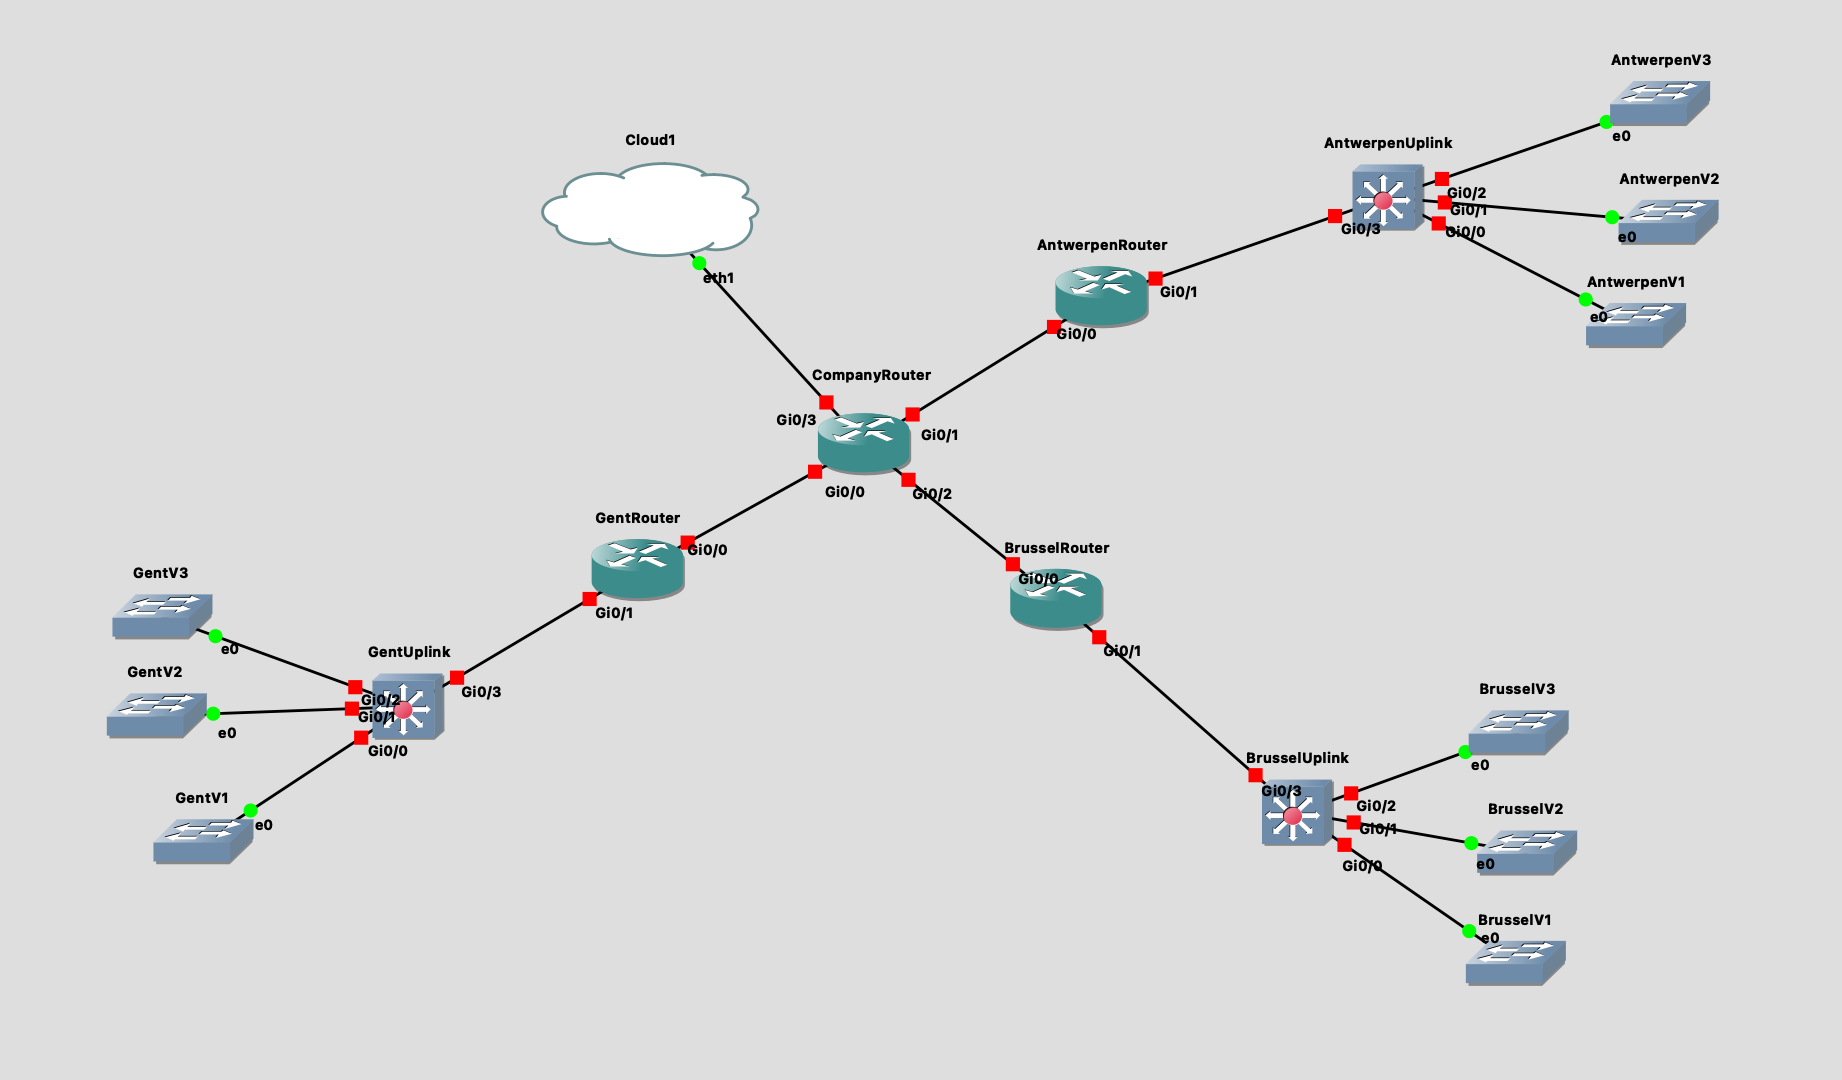
\includegraphics[width=0.5\textwidth]{../graphics/topologie.png}
  \caption{Netwerktopologie van de testomgeving}
\end{figure}

\section{Conclusies}

De resultaten tonen duidelijke voordelen van netwerkautomatisatie met Ansible:
\begin{itemize}
    \item \textbf{Tot 70\% tijdswinst} bij configuratie van meerdere toestellen
    \item Consistente en reproduceerbare configuraties
    \item Betere schaalbaarheid bij groeiende netwerken
    \item Minder kans op configuratiefouten
\end{itemize}

Een beperking van het onderzoek is het gebruik van een virtuele testomgeving.
Verder onderzoek op fysieke netwerkapparatuur is aangewezen.

\section{Toekomstig onderzoek}
Beginnen met PoC testen op fysieke netwerkapparatuur

Mogelijke uitbreidingen:
\begin{itemize}
    \item Gebruik van dynamische inventories
    \item Integratie met Git en CI/CD-pipelines
\end{itemize}

\end{multicols}
\end{document}